% mnras_template.tex 
%
% LaTeX template for creating an MNRAS paper
%
% v3.0 released 14 May 2015
% (version numbers match those of mnras.cls)
%
% Copyright (C) Royal Astronomical Society 2015
% Authors:
% Keith T. Smith (Royal Astronomical Society)

% Change log
%
% v3.0 May 2015
%    Renamed to match the new package name
%    Version number matches mnras.cls
%    A few minor tweaks to wording
% v1.0 September 2013
%    Beta testing only - never publicly released
%    First version: a simple (ish) template for creating an MNRAS paper

%%%%%%%%%%%%%%%%%%%%%%%%%%%%%%%%%%%%%%%%%%%%%%%%%%
% Basic setup. Most papers should leave these options alone.
\documentclass[fleqn,usenatbib]{mnras} 

% MNRAS is set in Times font. If you don't have this installed (most LaTeX
% installations will be fine) or prefer the old Computer Modern fonts, comment
% out the following line
\usepackage{newtxtext,newtxmath}
% Depending on your LaTeX fonts installation, you might get better results with one of these:
%\usepackage{mathptmx}
%\usepackage{txfonts}

% Use vector fonts, so it zooms properly in on-screen viewing software
% Don't change these lines unless you know what you are doing
\usepackage[T1]{fontenc}

% Allow "Thomas van Noord" and "Simon de Laguarde" and alike to be sorted by "N" and "L" etc. in the bibliography.
% Write the name in the bibliography as "\VAN{Noord}{Van}{van} Noord, Thomas"
\DeclareRobustCommand{\VAN}[3]{#2}
\let\VANthebibliography\thebibliography
\def\thebibliography{\DeclareRobustCommand{\VAN}[3]{##3}\VANthebibliography}


%%%%% AUTHORS - PLACE YOUR OWN PACKAGES HERE %%%%%

% Only include extra packages if you really need them. Common packages are:
\usepackage{graphicx}	% Including figure files
\usepackage{amsmath}	% Advanced maths commands
\usepackage{amssymb}	% Extra maths symbols

%%%%%%%%%%%%%%%%%%%%%%%%%%%%%%%%%%%%%%%%%%%%%%%%%%

%%%%% AUTHORS - PLACE YOUR OWN COMMANDS HERE %%%%%

% Please keep new commands to a minimum, and use \newcommand not \def to avoid
% overwriting existing commands. Example:
%\newcommand{\pcm}{\,cm$^{-2}$}	% per cm-squared

\usepackage[dvipsnames]{xcolor}
\newcommand{\fk}[1]{{\bf \textcolor{PineGreen}{#1}}}		% Florians edit 
%\definecolor{midblue}{rgb}{0.0,0.4,0.7}
%\definecolor{midgreen}{rgb}{0.1,0.6,0.3}
\definecolor{mypurple}{rgb}{0.7,0.3,0.8}
\newcommand{\fg}[1]{\textcolor{mypurple}{#1}}
%\newcommand{\fag}[1]{\textcolor{midblue}{FAG: #1}}
%\newcommand{\vdag}{(v)^\dagger}
%\newcommand\kf{k_{\rm f} }
\newcommand\SNr{\dot\sigma_{\rm sn}}
\newcommand\OSN{\Omega_{\rm sn}}
\newcommand\ESK{E_{\rm kin}}
\newcommand\EST{E_{\rm th}}
\newcommand\ESN{E_{\sigma}}
%\newcommand\Ms{M_{\rm s}}
\newcommand{\vect}[1]{{{\mbox{\boldmath $#1$}}}}%also makes bold Greek letters
\newcommand\kpc{~ {\rm kpc}}
\newcommand\pc{~ {\rm pc}}
\newcommand\dx{ {\delta x}}
\newcommand\Myr{~ {\rm Myr}}
\newcommand\erg{~ {\rm erg}}
\newcommand\kms{~ {\rm km~ s}^{-1}}
\def\cmcube{{\,{\rm cm}^{-3}}} 
\def\rmp{{Rev.~Mod.~Phys.}}             % Review of Modern Physics


%%%%%%%%%%%%%%%%%%%%%%%%%%%%%%%%%%%%%%%%%%%%%%%%%%

%%%%%%%%%%%%%%%%%%% TITLE PAGE %%%%%%%%%%%%%%%%%%%

% Title of the paper, and the short title which is used in the headers.
% Keep the title short and informative.
\title[Supernova induced processing of interstellar dust]{Supernova induced processing of interstellar dust}

% The list of authors, and the short list which is used in the headers.
% If you need two or more lines of authors, add an extra line using \newauthor
\author[L. Mattsson et al.]{
L. Mattsson,$^{1}$\thanks{E-mail: lars.mattsson@su.se}
Florian Kirchschlager,$^{2}$ and
Frederick A. Gent$^{3,4}$
\\
% List of institutions
$^{1}$Nordita, KTH Royal Institute of Technology and Stockholm University, Roslagstullsbacken 23, SE-106 91 Stockholm, Sweden\\
$^{2}$
Department
of Physics and Astronomy, University College London, Gower Street, London WC1E 6BT, UK\\
$^{3}$
Astroinformatics, Department of Computer Science, Aalto University, PO Box 15400, FI-00076 Aalto, Finland\\
$^{4}$
    School of Mathematics, Statistics and Physics,
      Newcastle University, NE1 7RU, UK 
}


% These dates will be filled out by the publisher
\date{Accepted XXX. Received YYY; in original form ZZZ}

% Enter the current year, for the copyright statements etc.
\pubyear{2021}

% Don't change these lines
\begin{document}
\label{firstpage}
\pagerange{\pageref{firstpage}--\pageref{lastpage}}
\maketitle

% Abstract of the paper
\begin{abstract}
This is a simple template for authors to write new MNRAS papers.
The abstract should briefly describe the aims, methods, and main results of the paper.
It should be a single paragraph not more than 250 words (200 words for Letters).
No references should appear in the abstract.
\end{abstract}

% Select between one and six entries from the list of approved keywords.
% Don't make up new ones.
\begin{keywords}
keyword1 -- keyword2 -- keyword3
\end{keywords}

%%%%%%%%%%%%%%%%%%%%%%%%%%%%%%%%%%%%%%%%%%%%%%%%%%

%%%%%%%%%%%%%%%%% BODY OF PAPER %%%%%%%%%%%%%%%%%%

\section{Introduction}
\fk{Test.}

\newpage~
\newpage
 %######################################################################################################################  %######################################################################################################################
 %###################################################################################################################### 
 
\section{Hydrodynamic simulations}\label{sect:HD}


  The simulations of dust are applied to a background ISM modelling the 
  hydrodynamics of an explosion of a supernova (SN). 
  Each model is within a 3D periodic domain large enough to evolve the SN
  remnant to the stage at which the leading blast wave slows to the local
  sound speed of the ambient ISM.
  We model an ISM with mean ambient gas number density either $n_0=0.1,$ or
  $1\cmcube$, with the ISM either uniform at rest or subject to background
  turbulence.
  The models have an equidistant grid resolution of 0.5 and 0.25\,pc along each
  edge, sufficiently well resolved to obtain well converged solutions 
  \citep{GMKSH20,GMKS21} and also to exhibit instabilities resembling 
  Vishniac-Ostriker-Bertschinger overstability \citep{Vishniac83,VOB85} or
  potentially Richtmyer-Meshkov instability \citep{Bro02}.


  The SN remnant is initialised by the injection of thermal energy 
  $\EST = 10^{51}\erg$ within a sphere of initial nominal radius of {$R_0$}, 
  following a radial profile as 
  \begin{equation}  
     E(R) = E_0\exp\left(-\left[
     R/{R_0}
  \right]^{{2}}\right),
  \end{equation}
  with normalising coefficient $E_0$ set such that the volume integral of
  $E(R)=\EST$.
  The remnant origin is located on a grid point, and $R_0 = 5$\,pc for
  grid resolution 0.5\,pc.
  The initial condition creates a blast wave, which rapidly evacuates the ISM
  from the origin of the sphere and continues to expand into the ambient ISM.
  Within a short time, still within the adiabatic expansion phase of the 
  SN lifespan, the properties of the remnant converge to a solution fitting
  the Sedov-Taylor analytic solution \citep{Taylor50,Sedov59},
  \begin{equation}
    \label{eq:sed}
    R= \left(\kappa\frac{\EST}{\rho_{0}}\right)^{{1}/{5}}t^{{2}/{5}},
  \end{equation}
  where $R$ is the remnant radius, $\EST$ the explosion energy, $\rho_{0}$ the
  ambient gas density, and the dimensionless parameter $\kappa\approx2.026$ for
  $\gamma=5/3$ \citep{Ostriker88}.
  We neglect any additional mass from the SN ejecta.

 Non-adiabatic heating $\Gamma$ and cooling $\Lambda (T)$ are included
 \citep{Gent:2013b}.
 Cooling by radiative losses follow \citet{Wolfire:1995} and
 \citet{Sarazin:1987}, using a piecewise power law dependence of the cooling
 coefficient on temperature.
 The contribution from FUV heating follows
 \citet[][see \citep{Gent:2013a}]{Wolfire:1995}, which is truncated for
 temperatures above 10$^{4}$\,K.
 When radiative cooling processes are included the SN evolution changes.
 As the remnant expands and the shock front accumulates more gas from the
 ambient ISM, cooling becomes more efficient in the increasingly dense shell.
 Loss of energy more rapidly reduces the shell speed.  
 As demonstrated by \citet{GMKSH20} at resolution better than 1\,pc our 
 solution converges to the semi-analytical non-adiabatic solutions obtained by 
 \citet{Cioffi88}, slightly modified to account for cooling in our model
 continuing to apply for $T<10^4$\,K.

 To integrate these solutions we use the Pencil
 Code\footnote{https://github.com/pencil-code} \citep{Pencil-JOSS} for
 the system of non-ideal, compressible, non-isothermal HD equations
%-------------------------------------------------------------------------------
  \begin{eqnarray}
  \label{eq:mass}
    \frac{D\rho}{Dt} &=& 
    -\rho \vect\nabla \cdot \vect{u}
    +\vect\nabla \cdot\zeta_D\vect\nabla\rho,
  \end{eqnarray}
%-------------------------------------------------------------------------------
  \begin{eqnarray}
  \label{eq:mom}
    \rho\frac{D\vect{u}}{Dt} &=& 
    %\vect\nabla{\ESK\sigma}
    -\rho c_{\rm s}^2\vect\nabla\left({s}/{c_{\rm p}}+\ln\rho\right)
    %+\vect{j}\times\vect{B}
    \nonumber\\
    &+&\vect\nabla\cdot \left(2\rho\nu{\mathbfss W}\right)
    +\rho\,\vect\nabla\left(\zeta_{\nu}\vect\nabla \cdot \vect{u} \right)
    \nonumber\\
    &+&\vect\nabla\cdot \left(2\rho\nu_3{\mathbfss W}^{(3)}\right)
  {-\vect u\vect{\nabla}\cdot\left(\zeta_D\vect{\nabla}\rho\right)},
  \end{eqnarray}
%-------------------------------------------------------------------------------
  \begin{eqnarray}
  \label{eq:ent}
    \rho T\frac{D s}{Dt} &=&
     \EST\dot\sigma +\rho\Gamma
    -\rho^2\Lambda %+\eta\mu_0\vect{j}^2 
    \nonumber\\
    &+&2 \rho \nu\left|{\mathbfss W}\right|^{2}
    +\rho\,\zeta_{\nu}\left(\vect\nabla \cdot \vect{u} \right)^2
    \nonumber\\
    &+&\vect\nabla\cdot\left(\zeta_\chi\rho T\vect\nabla s\right)
    +\rho T\chi_3\vect\nabla^6 s
    \nonumber\\
    &-& {c_{\rm{v}}\,T \left(
    \zeta_D\nabla^2\rho + \vect\nabla\zeta_D\cdot\vect\nabla\rho\right)},
  \end{eqnarray}
%%-------------------------------------------------------------------------------
%  \begin{eqnarray}
%  \label{eq:ind}
%    \frac{\partial \vect{A}}{\partial t} &=&
%    \vect{u}\times\vect{B}
%    +\eta\vect\nabla^2\vect{A}
%    +\eta_3\vect\nabla^6\vect{A},
%  \end{eqnarray}
%%-------------------------------------------------------------------------------
 with the ideal gas equation of state closing the system.
 Most variables take their usual meanings.
 \fg{Lars, please check the numbers are correct}
 Terms containing $\zeta_D{=2.5},\,\zeta_\nu{=6.5}$ and $\zeta{_\chi=2.5}$
 are applied to resolve shock discontinuities with artificial diffusion of
 mass, momentum, and energy proportional to shock strength
 \citep[see][for details]{GMKSH20}.
 Equations~\eqref{eq:mom} and \eqref{eq:ent} include terms with $\zeta_D$
 to provide momentum and energy conserving corrections for the
 artificial mass diffusion applying in Equation~\eqref{eq:mass}.
 Terms containing $\nu_3,\,\chi_3$ and $\eta_3$ apply sixth-order hyperdiffusion
 to resolve grid-scale instabilities \citep[see, e.g.,][]{ABGS02,HB04,GMKS21},
 with mesh Reynolds number set to be $\simeq1$ for each $\dx$.
 The incidence of SN denoted by $\dot\sigma$ is once at $t=0$.


 \begin{table}
 \centering
 \caption{List of hydrodynamics simulations}
 \begin{tabular}{ l l l}
 \hline\hline
 Index&Note&\\\hline 
 A&$n_\text{gas}=0.1\,\text{cm}^{-3}$, no turbulence&\\\hline  
 B&$n_\text{gas}=1.0\,\text{cm}^{-3}$, no turbulence&\\\hline   
 C&$n_\text{gas}=0.1\,\text{cm}^{-3}$, turbulence&\\\hline  
 D&$n_\text{gas}=1.0\,\text{cm}^{-3}$, turbulence&\\\hline   
 \end{tabular}
 \label{List_hydrosimulations}
 \end{table}

\newpage~
\newpage
 %######################################################################################################################  %######################################################################################################################
 %###################################################################################################################### 
\section{Dust processing}
 \begin{table}
 \centering
 \caption{List of dust post-processing simulations}
 \begin{tabular}{ l l l}
 \hline\hline
 Index&Note&\\\hline 
 1&Only transport&\\\hline  
 2&Transport + Sputtering + Grain-grain collisions&\\\hline 
 \end{tabular}
 \label{List_Dustsimulations}
 \end{table}
 
    \begin{figure*}
 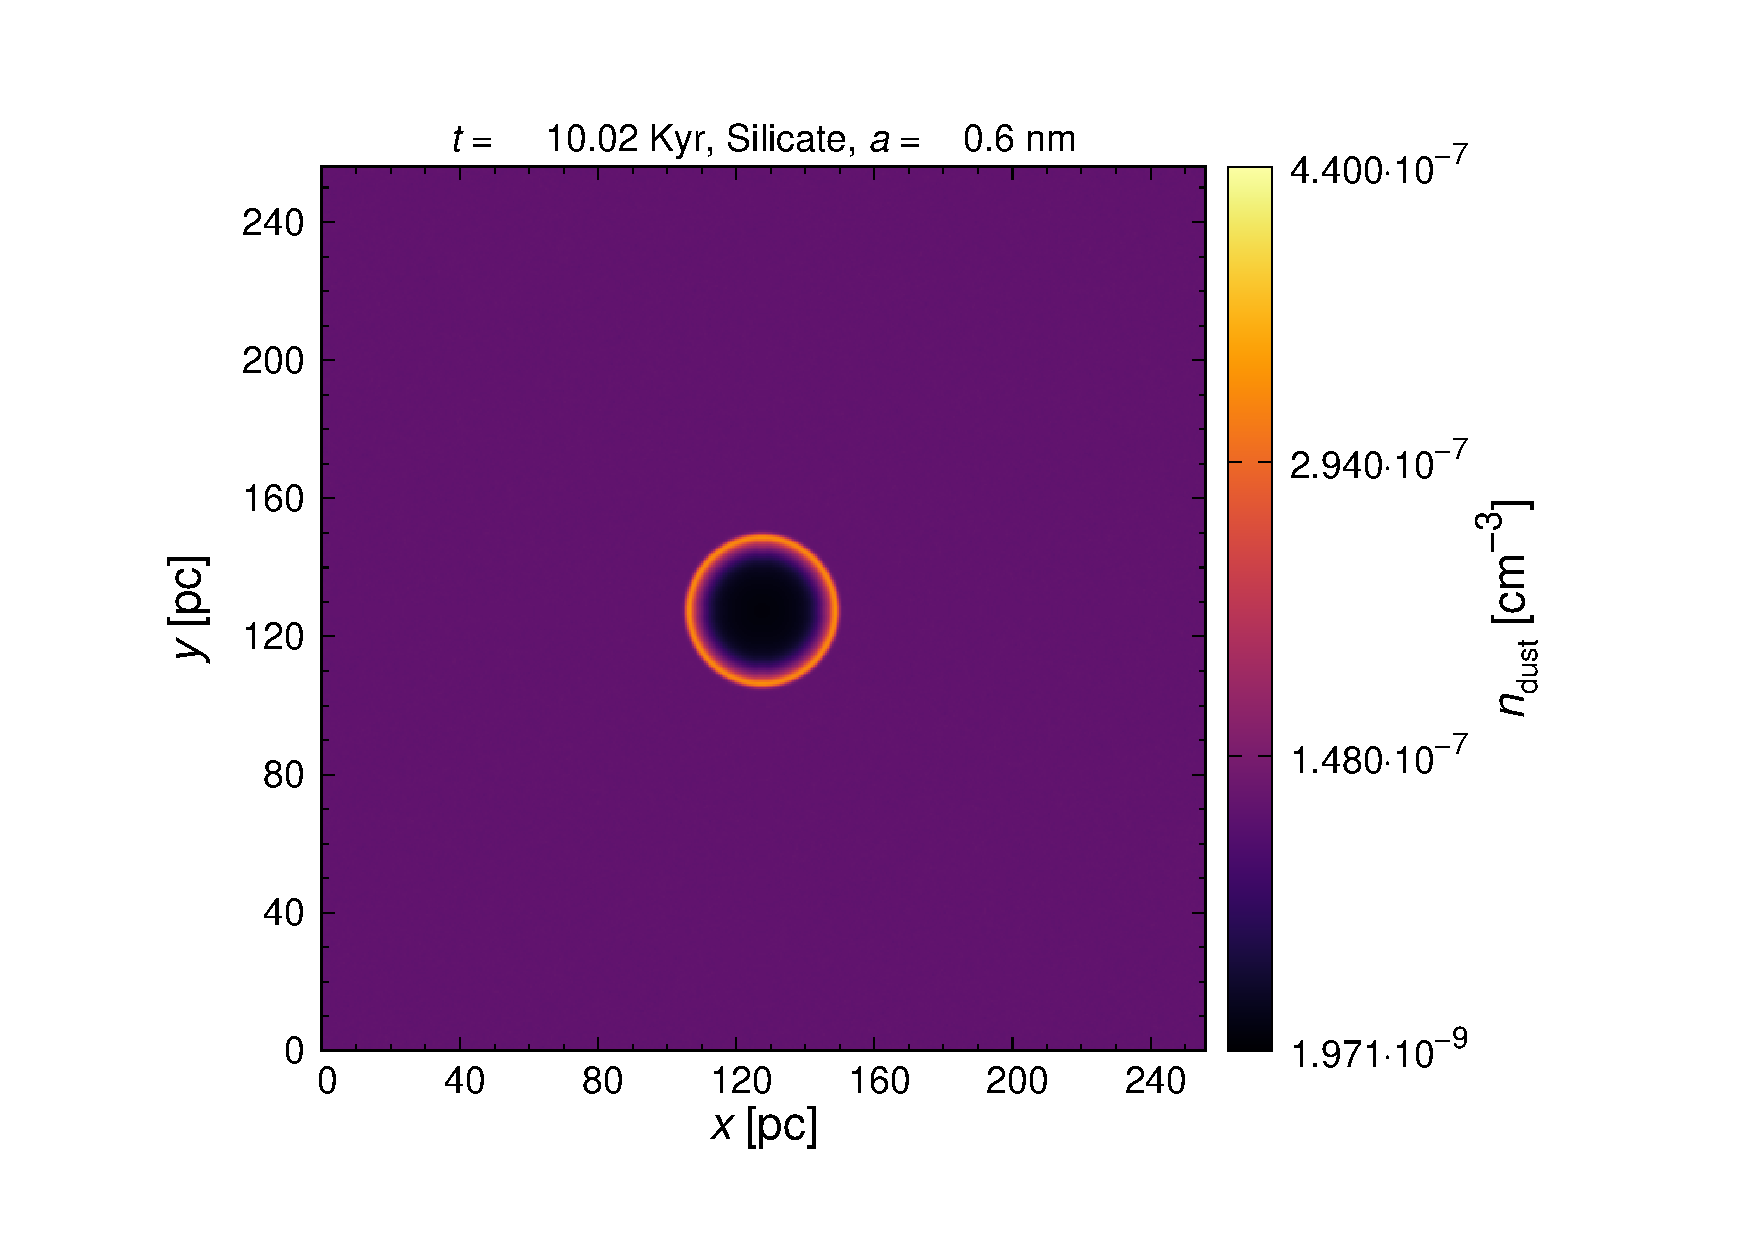
\includegraphics[trim=2.8cm 1.5cm 9.3cm 2.0cm, clip=true,page=1,height = 4.5cm]{Pics/Pics_C1/Density_1_00041.pdf}\hspace*{-0.1cm}
 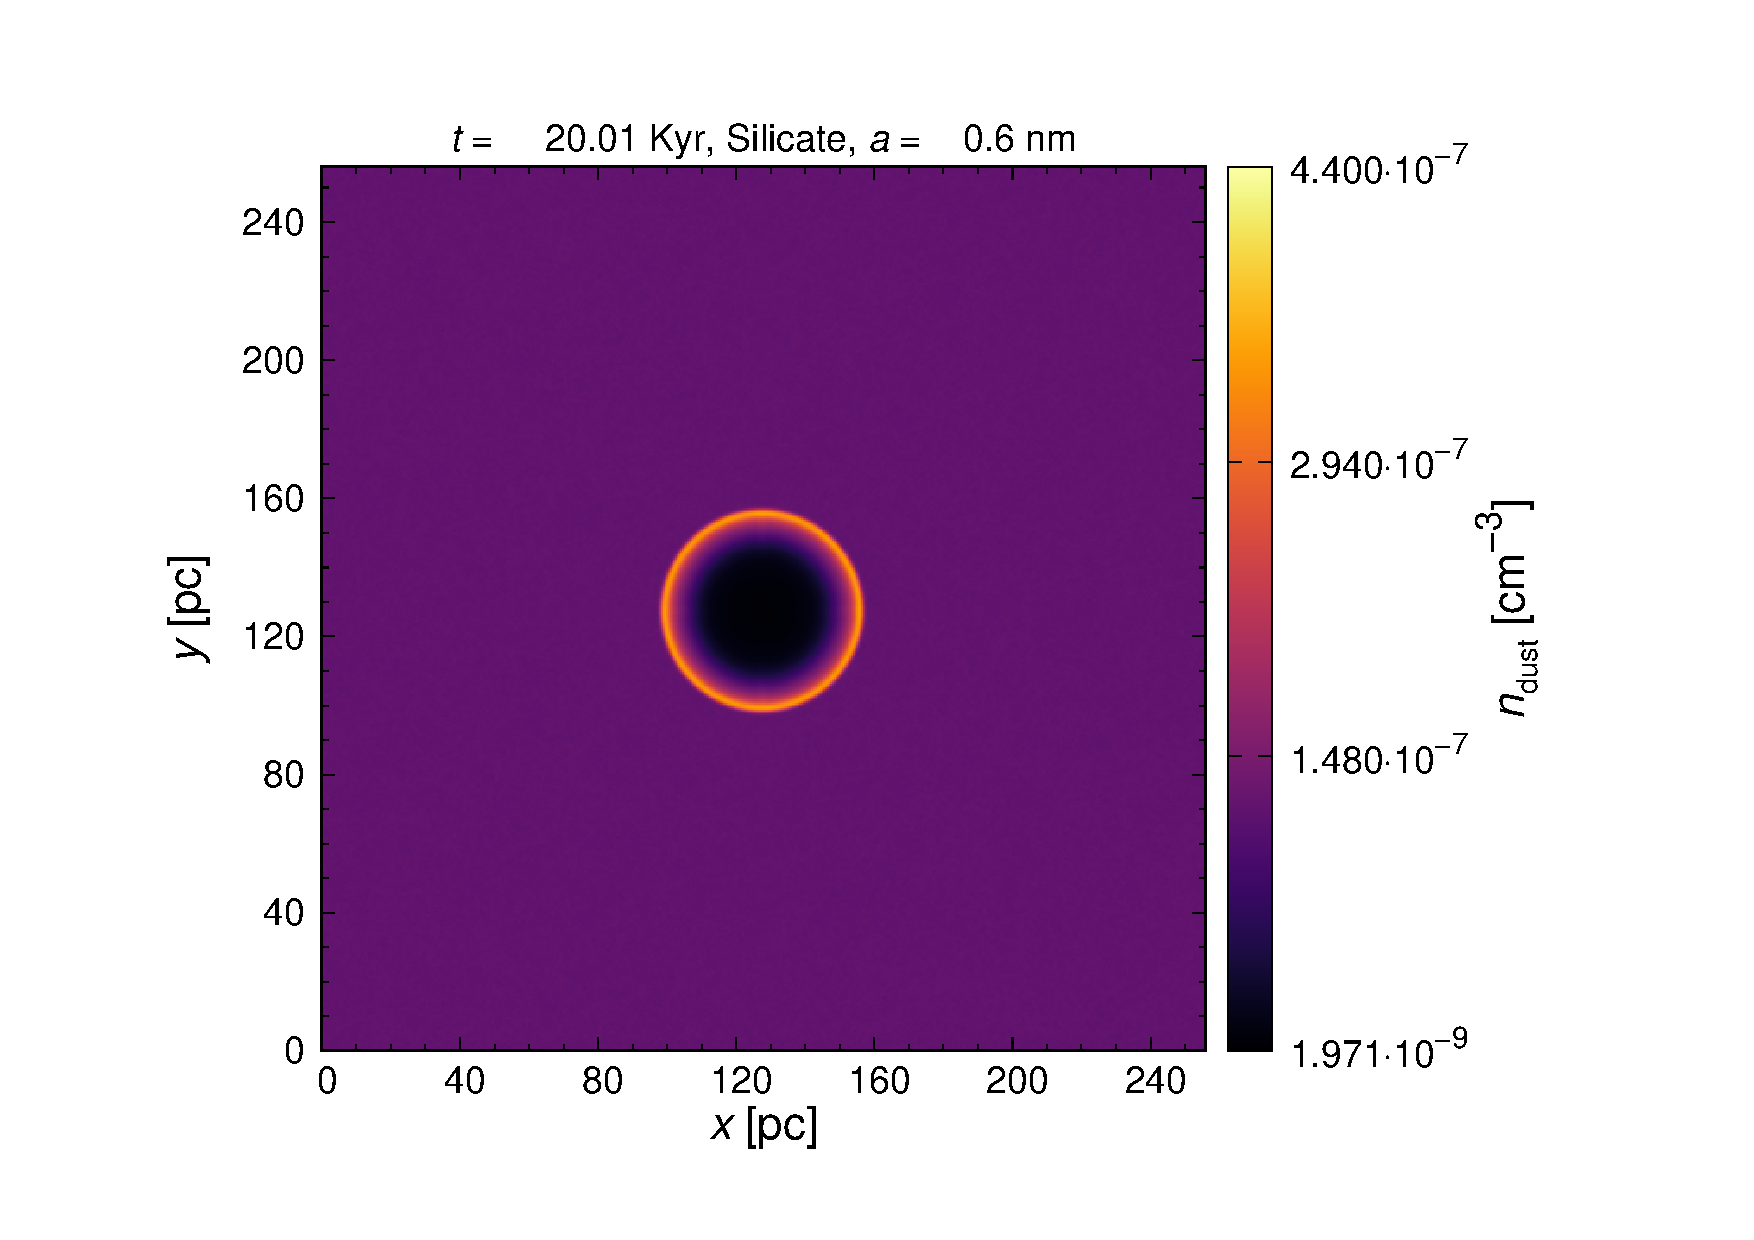
\includegraphics[trim=5.2cm 1.5cm 9.3cm 2.0cm, clip=true,page=1,height = 4.5cm]{Pics/Pics_C1/Density_1_00081.pdf}\hspace*{-0.1cm}
 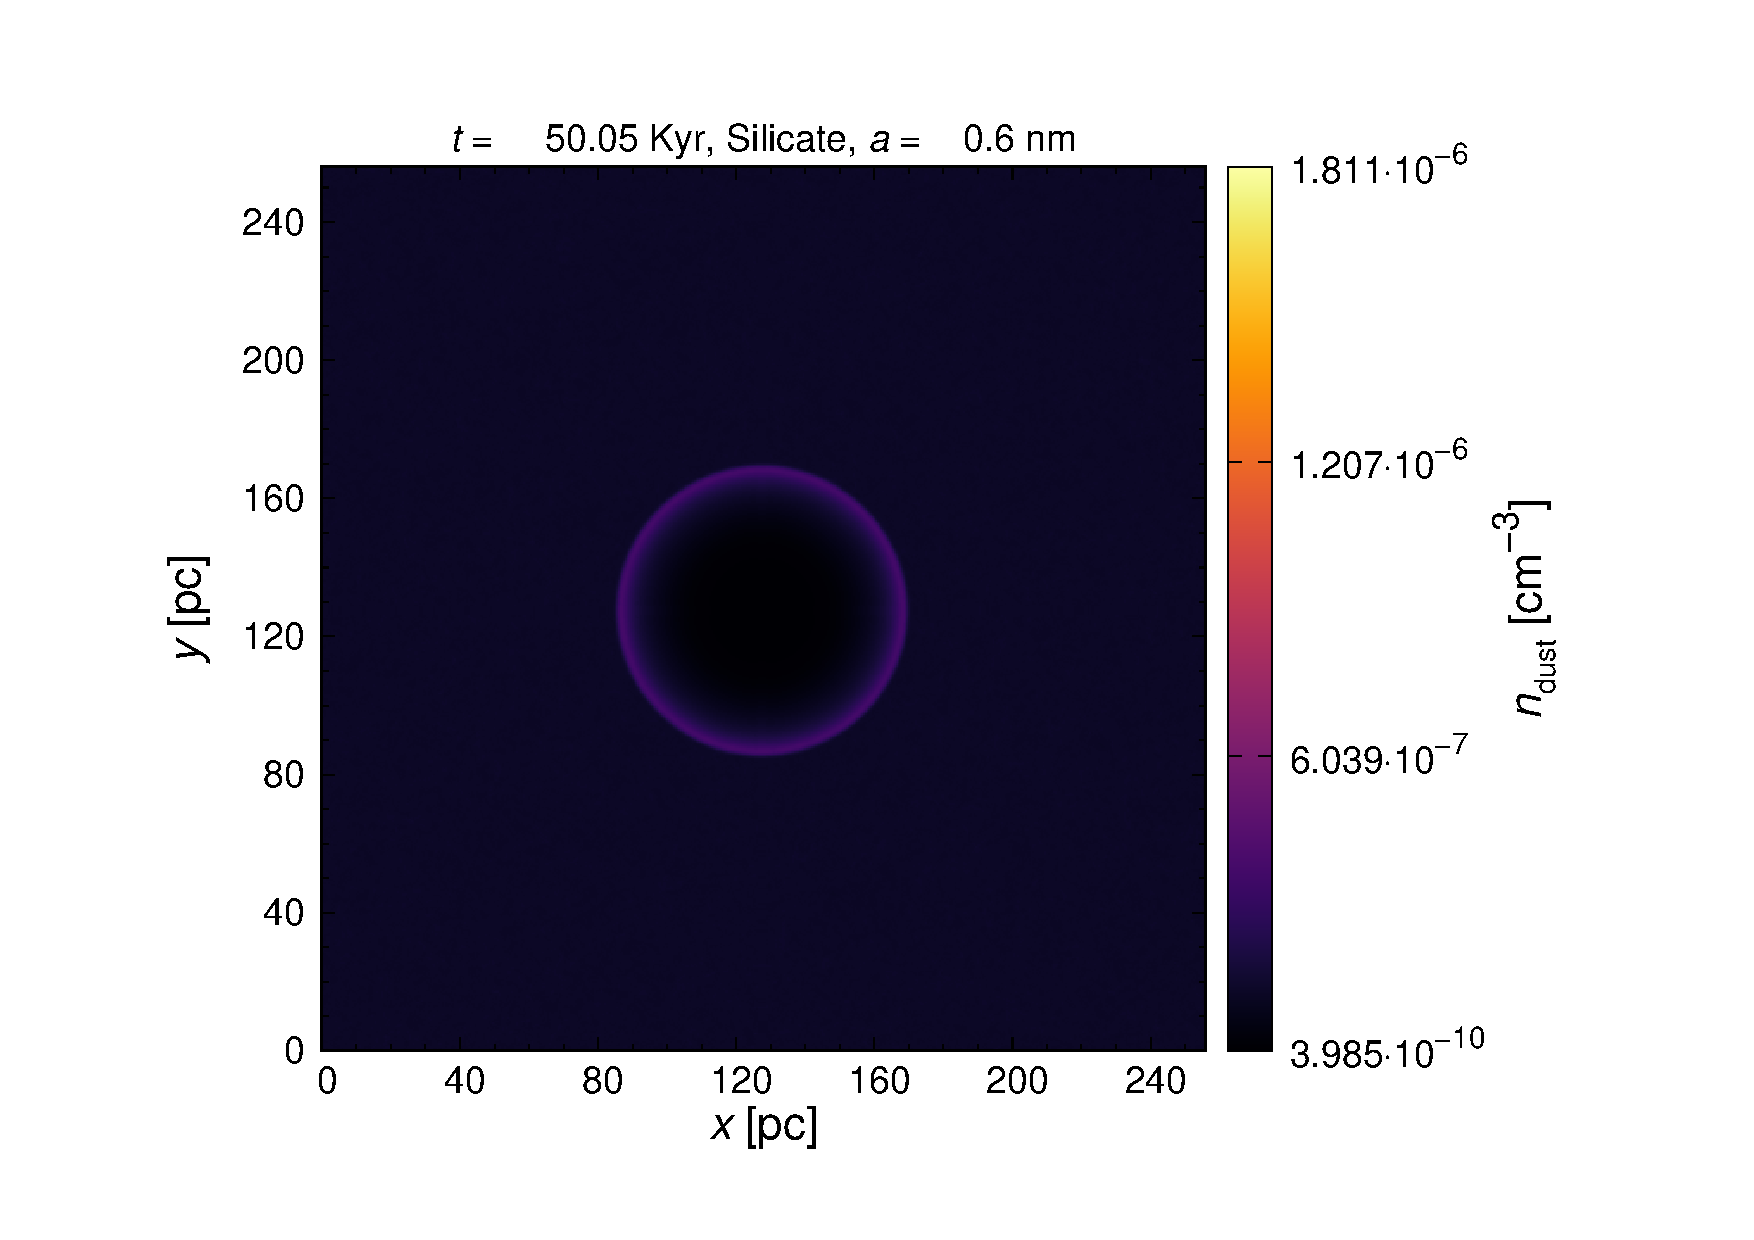
\includegraphics[trim=5.2cm 1.5cm 9.3cm 2.0cm, clip=true,page=1,height = 4.5cm]{Pics/Pics_C1/Density_1_00201.pdf}\hspace*{-0.1cm}
 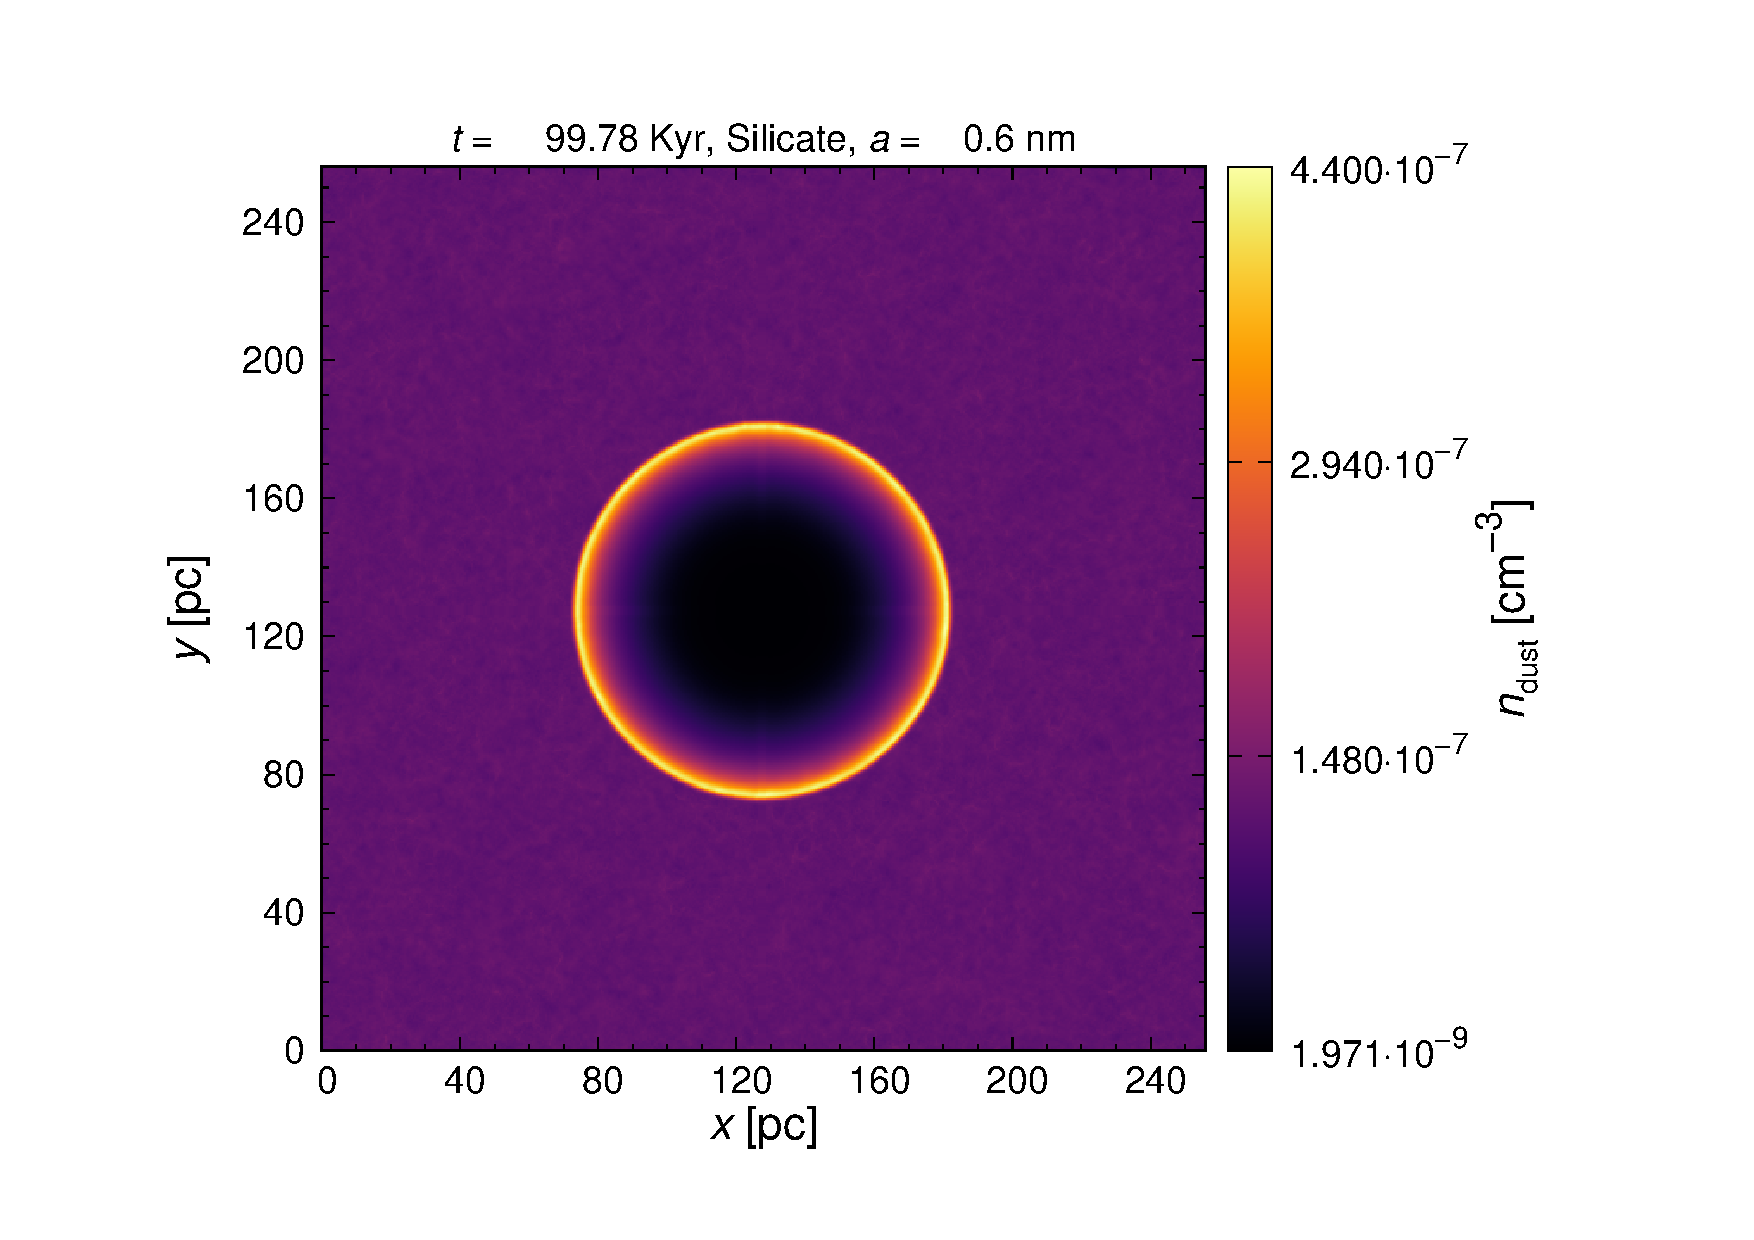
\includegraphics[trim=5.2cm 1.5cm 3.2cm 2.0cm, clip=true,page=1,height = 4.5cm]{Pics/Pics_C1/Density_1_00400.pdf}\\
  \includegraphics[trim=2.8cm 1.5cm 9.3cm 2.0cm, clip=true,page=2,height = 4.5cm]{Pics/Pics_C1/Density_1_00041.pdf}\hspace*{-0.1cm}
 \includegraphics[trim=5.2cm 1.5cm 9.3cm 2.0cm, clip=true,page=2,height = 4.5cm]{Pics/Pics_C1/Density_1_00081.pdf}\hspace*{-0.1cm}
 \includegraphics[trim=5.2cm 1.5cm 9.3cm 2.0cm, clip=true,page=2,height = 4.5cm]{Pics/Pics_C1/Density_1_00201.pdf}\hspace*{-0.1cm}
 \includegraphics[trim=5.2cm 1.5cm 3.2cm 2.0cm, clip=true,page=2,height = 4.5cm]{Pics/Pics_C1/Density_1_00400.pdf}\\
  \includegraphics[trim=2.8cm 1.5cm 9.3cm 2.0cm, clip=true,page=3,height = 4.5cm]{Pics/Pics_C1/Density_1_00041.pdf}\hspace*{-0.1cm}
 \includegraphics[trim=5.2cm 1.5cm 9.3cm 2.0cm, clip=true,page=3,height = 4.5cm]{Pics/Pics_C1/Density_1_00081.pdf}\hspace*{-0.1cm}
 \includegraphics[trim=5.2cm 1.5cm 9.3cm 2.0cm, clip=true,page=3,height = 4.5cm]{Pics/Pics_C1/Density_1_00201.pdf}\hspace*{-0.1cm}
 \includegraphics[trim=5.2cm 1.5cm 3.2cm 2.0cm, clip=true,page=3,height = 4.5cm]{Pics/Pics_C1/Density_1_00400.pdf}\\
  \includegraphics[trim=2.8cm 1.5cm 9.3cm 2.0cm, clip=true,page=4,height = 4.5cm]{Pics/Pics_C1/Density_1_00041.pdf}\hspace*{-0.1cm}
 \includegraphics[trim=5.2cm 1.5cm 9.3cm 2.0cm, clip=true,page=4,height = 4.5cm]{Pics/Pics_C1/Density_1_00081.pdf}\hspace*{-0.1cm}
 \includegraphics[trim=5.2cm 1.5cm 9.3cm 2.0cm, clip=true,page=4,height = 4.5cm]{Pics/Pics_C1/Density_1_00201.pdf}\hspace*{-0.1cm}
 \includegraphics[trim=5.2cm 1.5cm 3.2cm 2.0cm, clip=true,page=4,height = 4.5cm]{Pics/Pics_C1/Density_1_00400.pdf}\\
  \caption{Temporal evolution of the spatial dust density for \textbf{Simulation C-1} ($n_\text{gas}=0.1\,\text{cm}^{-3}$, turbulence, only dust transport). The first, second, third, and fourth rows show the distribution of 0.6, 6, 60, 600 nm grains, respectively. The colorscale is fixed for each row.}
  \end{figure*}  
 
\newpage~
\newpage~
\newpage~
\newpage
 %######################################################################################################################  %######################################################################################################################
 %###################################################################################################################### 
\section{Results and discussion}

   \begin{figure*}
        \resizebox{\hsize}{!}{
      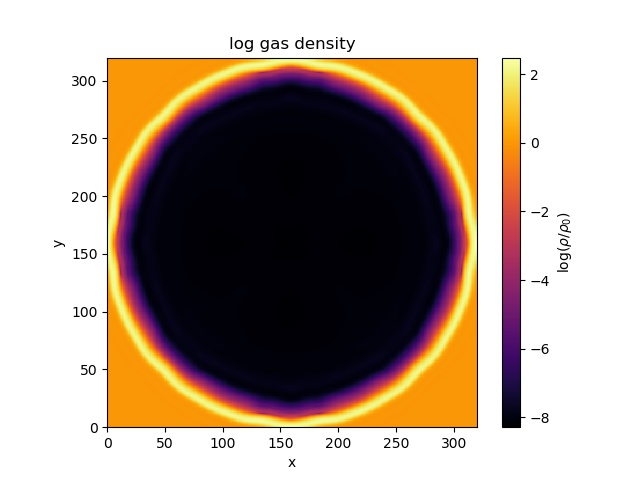
\includegraphics{3Dsedov_SN_dust_newsetup2_10pc_chi4_320_FGupd_rhoVAR60.jpg}
      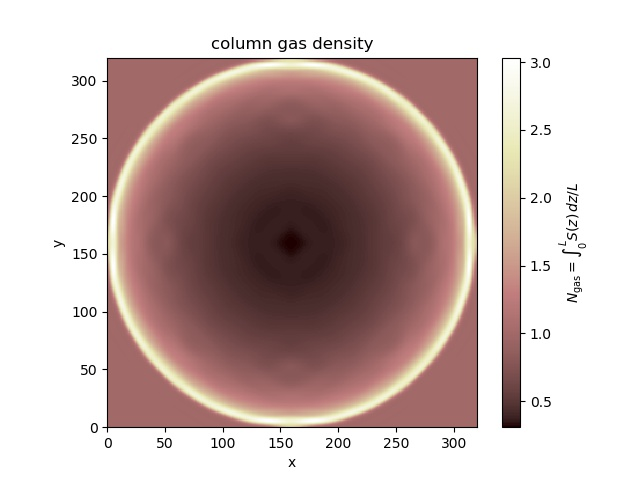
\includegraphics{3Dsedov_SN_dust_newsetup2_10pc_chi4_320_FGupd_column_gasVAR60.jpg}}
      \resizebox{\hsize}{!}{
      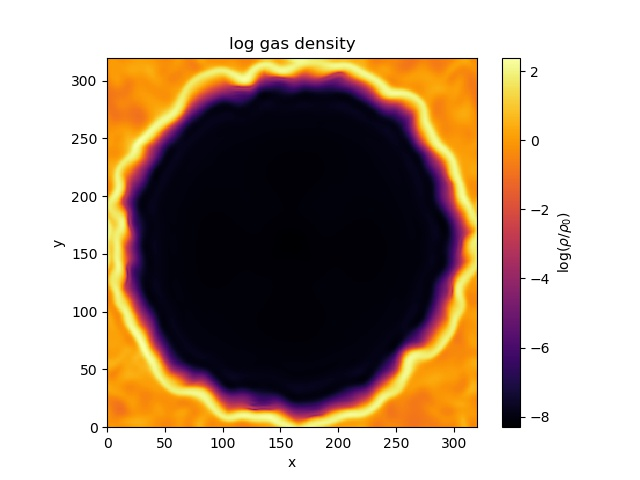
\includegraphics{3Dsedov_SN_dust_newsetup2_10pc_chi4_320_FGupd_uin2_rhoVAR60.jpg}
      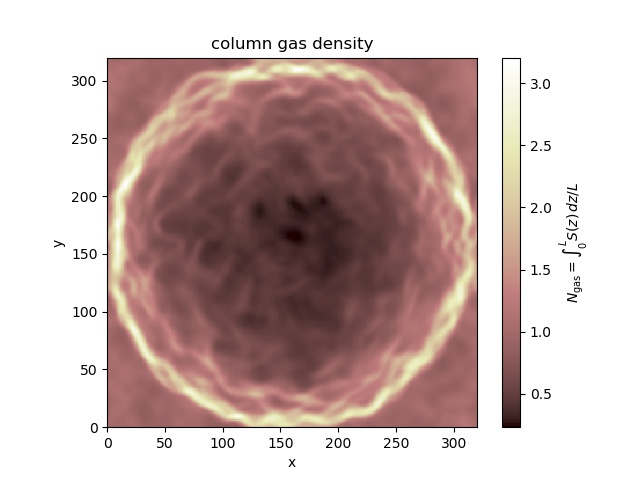
\includegraphics{3Dsedov_SN_dust_newsetup2_10pc_chi4_320_FGupd_uin2_column_gasVAR60.jpg}}

  \caption{\label{3Dsedov} }
  \end{figure*}  

  \begin{figure*}
        \resizebox{\hsize}{!}{
      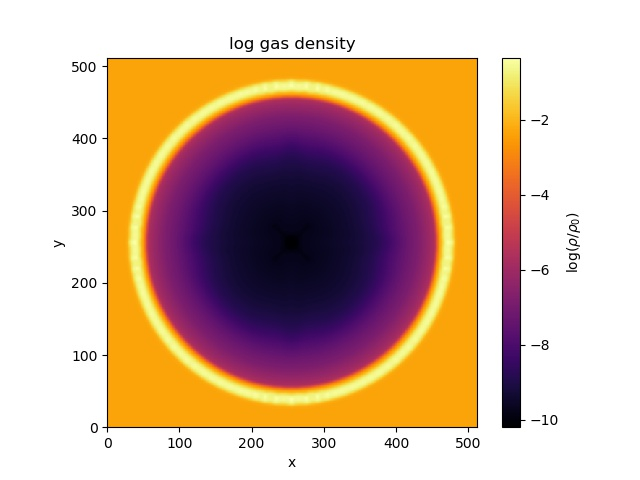
\includegraphics{3Dsedov_SN_dust_newsetup2_10pc_chi4_512_FGupd_new_n01_rhoVAR20.jpg}
      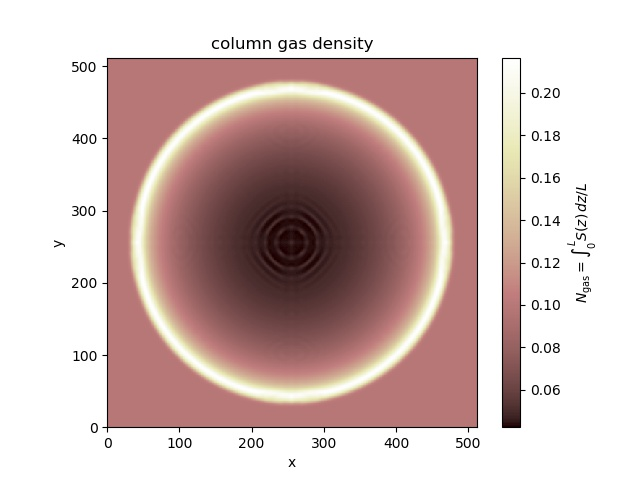
\includegraphics{3Dsedov_SN_dust_newsetup2_10pc_chi4_512_FGupd_new_n01_column_gasVAR20.jpg}}
      \resizebox{\hsize}{!}{
      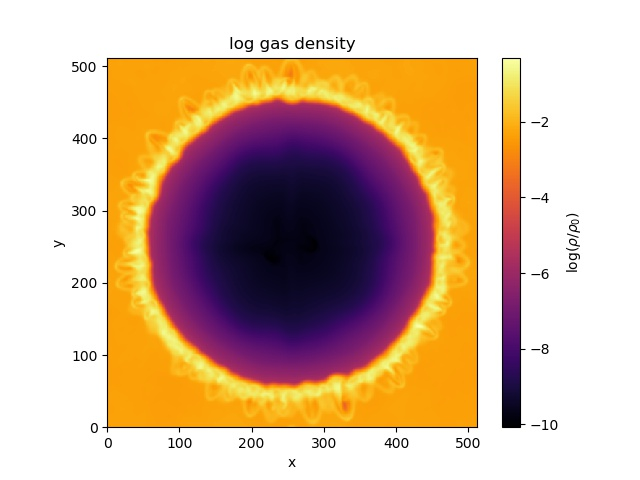
\includegraphics{3Dsedov_SN_dust_newsetup2_10pc_chi4_512_FGupd_new_n01_uin2_rhoVAR20.jpg}
      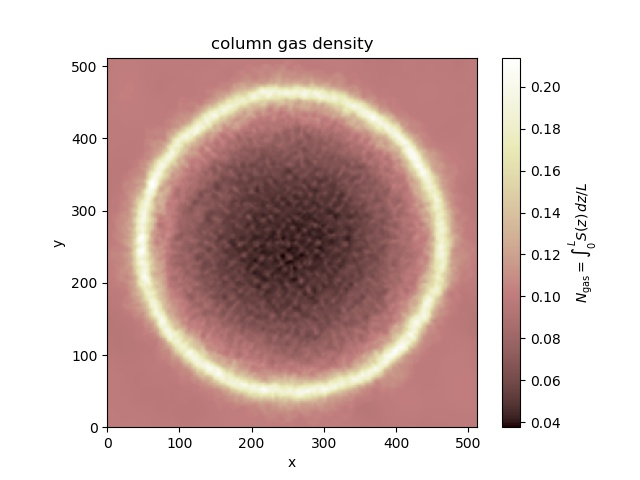
\includegraphics{3Dsedov_SN_dust_newsetup2_10pc_chi4_512_FGupd_new_n01_uin2_column_gasVAR20.jpg}}

  \caption{\label{3Dsedov} }
  \end{figure*} 

\section{Conclusions}


\section*{Acknowledgements}

The Acknowledgements section is not numbered. Here you can thank helpful
colleagues, acknowledge funding agencies, telescopes and facilities used etc.
Try to keep it short.

%%%%%%%%%%%%%%%%%%%%%%%%%%%%%%%%%%%%%%%%%%%%%%%%%%
\section*{Data Availability}

 
The inclusion of a Data Availability Statement is a requirement for articles published in MNRAS. Data Availability Statements provide a standardised format for readers to understand the availability of data underlying the research results described in the article. The statement may refer to original data generated in the course of the study or to third-party data analysed in the article. The statement should describe and provide means of access, where possible, by linking to the data or providing the required accession numbers for the relevant databases or DOIs.




%%%%%%%%%%%%%%%%%%%% REFERENCES %%%%%%%%%%%%%%%%%%

% The best way to enter references is to use BibTeX:

\bibliographystyle{mnras}
\bibliography{refs} % if your bibtex file is called example.bib


% Alternatively you could enter them by hand, like this:
% This method is tedious and prone to error if you have lots of references
%\begin{thebibliography}{99}
%\bibitem[\protect\citeauthoryear{Author}{2012}]{Author2012}
%Author A.~N., 2013, Journal of Improbable Astronomy, 1, 1
%\bibitem[\protect\citeauthoryear{Others}{2013}]{Others2013}
%Others S., 2012, Journal of Interesting Stuff, 17, 198
%\end{thebibliography}

%%%%%%%%%%%%%%%%%%%%%%%%%%%%%%%%%%%%%%%%%%%%%%%%%%

%%%%%%%%%%%%%%%%% APPENDICES %%%%%%%%%%%%%%%%%%%%%

\appendix

\section{Some extra material}

If you want to present additional material which would interrupt the flow of the main paper,
it can be placed in an Appendix which appears after the list of references.

%%%%%%%%%%%%%%%%%%%%%%%%%%%%%%%%%%%%%%%%%%%%%%%%%%


% Don't change these lines
\bsp	% typesetting comment
\label{lastpage}
\end{document}

% End of mnras_template.tex
